	\documentclass[12pt]{article}

%% Language and font encodings
\usepackage[english]{babel}
\usepackage[utf8x]{inputenc}
\usepackage[T1]{fontenc}

%% Sets page size and margins
\usepackage[a4paper,top=2cm,bottom=2cm,left=2cm,right=2.5cm,marginparwidth=1.75cm]{geometry}

%% Useful packages
\usepackage{amsmath}
\usepackage{amsfonts}
\usepackage{graphicx}
\usepackage[colorinlistoftodos]{todonotes}
\usepackage[colorlinks=true, allcolors=blue]{hyperref}

\title{Homework 6}
\author{Motoaki Takahashi}
\date{}

\begin{document}
\maketitle
\section*{Question 1}
Given the initial stock of lumber $k_{0}$, let $\mathcal{K}=[0, k_{0}]$ be the set of possible values for a stock of lumber, and  let $\mathcal{P}=\mathbb{R}$ be the set of possible prices. $\mathcal{K}\times\mathcal{P}$ is the state space. Let $(k, p)\in\mathcal{K}\times\mathcal{P}$. Then the Bellman equation is
\begin{equation}
    V(k, p)=\max_{k'} p\cdot (k-k')-0.2(k-k')^{1.5}+\delta\mathbb{E}_{p'\mid p}V(k', p')
\end{equation}
subject to
$$
p'=p_{0}+\rho p+u,\, u\sim N(0, \sigma_{u}^{2}),
$$
and
$$
k'\in[0, k].
$$
\section*{Question 2}
The vector of grids is $(0.6536,    0.6882,    0.7229,    0.7575,    0.7922,    0.8268,    0.8614, \cdots, 1.3118,    1.3464)$.
\clearpage
\section*{Question 3}
\begin{figure}[h]
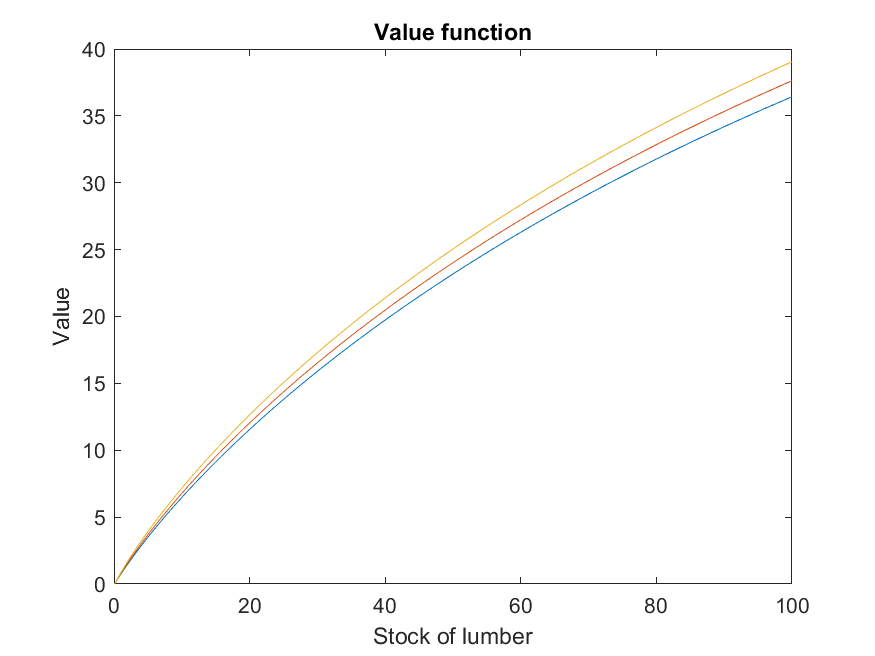
\includegraphics[width=\textwidth]{vf.png}
\caption{The values as a function of lumber stocks, for $p=0.9, 1, 1.1$}
\end{figure}
\clearpage
\section*{Question 4}

\begin{figure}[h]
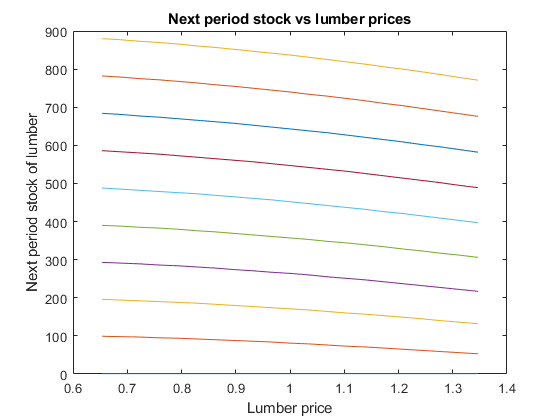
\includegraphics[width=\textwidth]{nextstock.png}
\caption{Next period optimal stocks as a function of lumber prices, for current period stock 0.1, 10.1, 20.1, ..., 90.1}
\end{figure}

\clearpage
\section*{Question 5}
\begin{figure}[h]
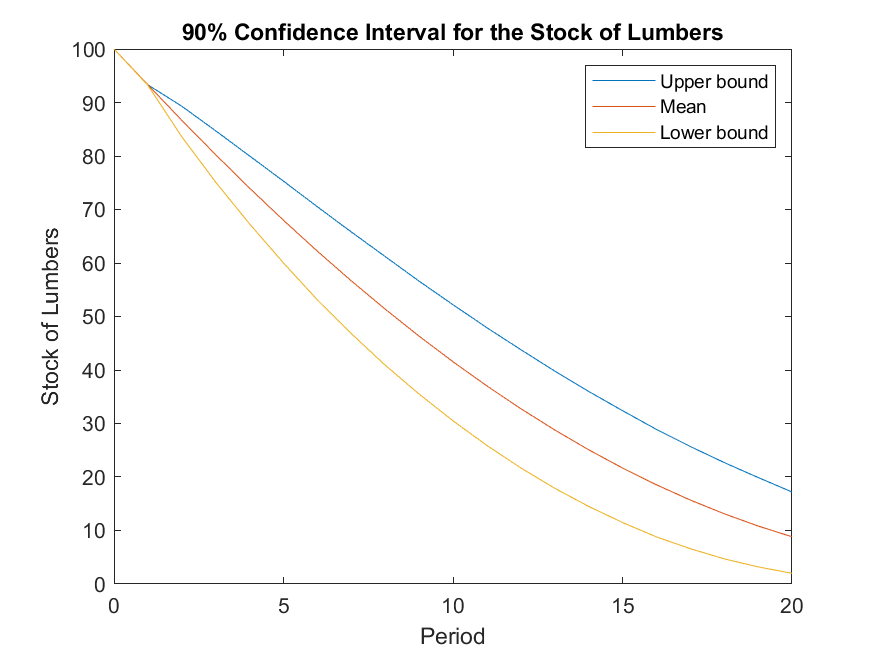
\includegraphics[width=\textwidth]{ci.png}
\caption{Expected stock and 90\% confidence interval}
\end{figure}
\clearpage
\section*{Question 6}
Since $p=0.9, 1.1$ are not on the grid, I draw two curves associated with the closest prices to them in Fig. 4.
\begin{figure}[h]
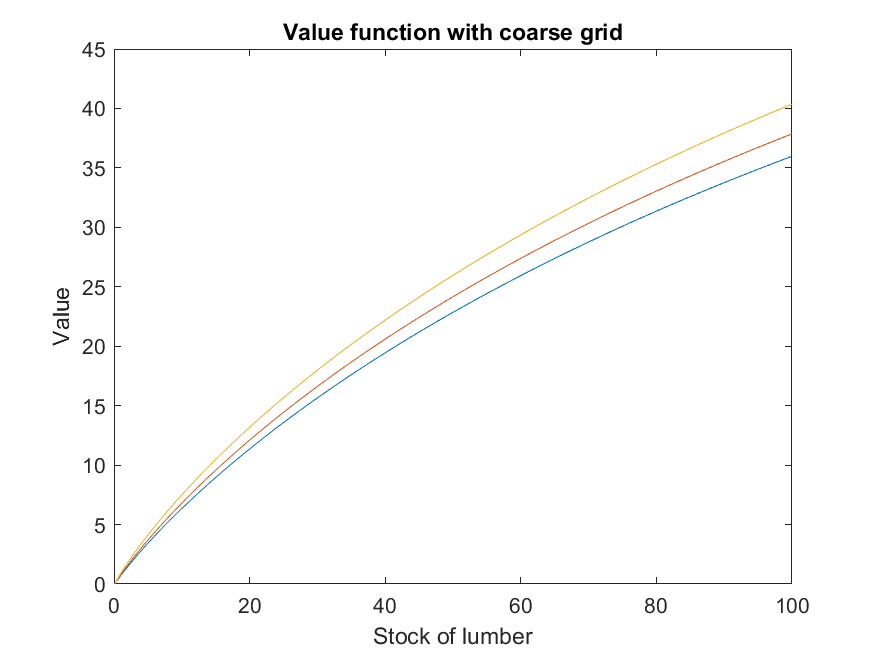
\includegraphics[width=\textwidth]{vf2.png}
\caption{The values as a function of lumber stocks, for $p=0.827, 1, 1.173$}
\end{figure}
\clearpage
\begin{figure}
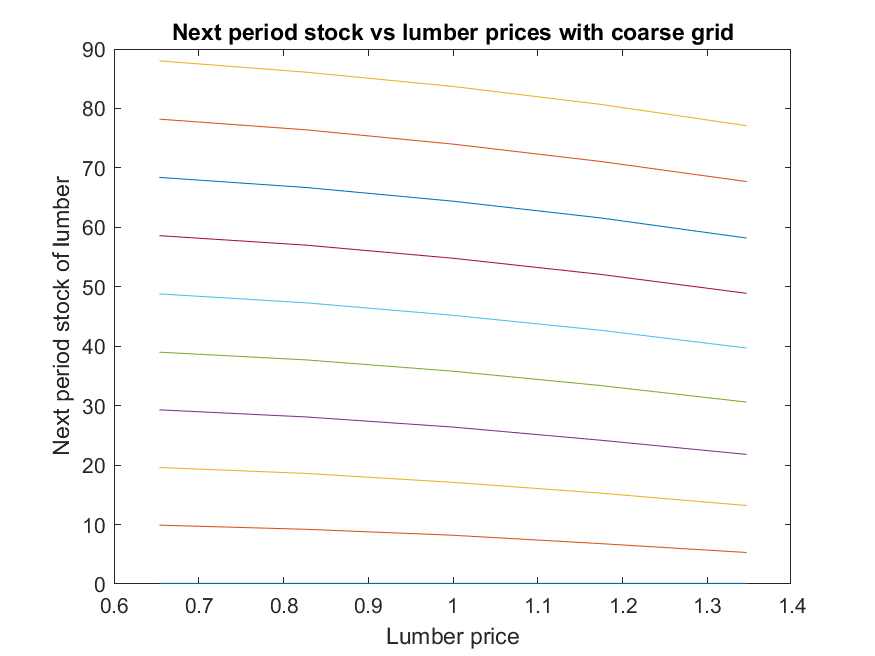
\includegraphics[width=\textwidth]{nextstock2.png}
\caption{Next period optimal stocks as a function of lumber prices, for current period stock 0.1, 10.1, 20.1, ..., 90.1}
\end{figure}
\clearpage
\begin{figure}[h]
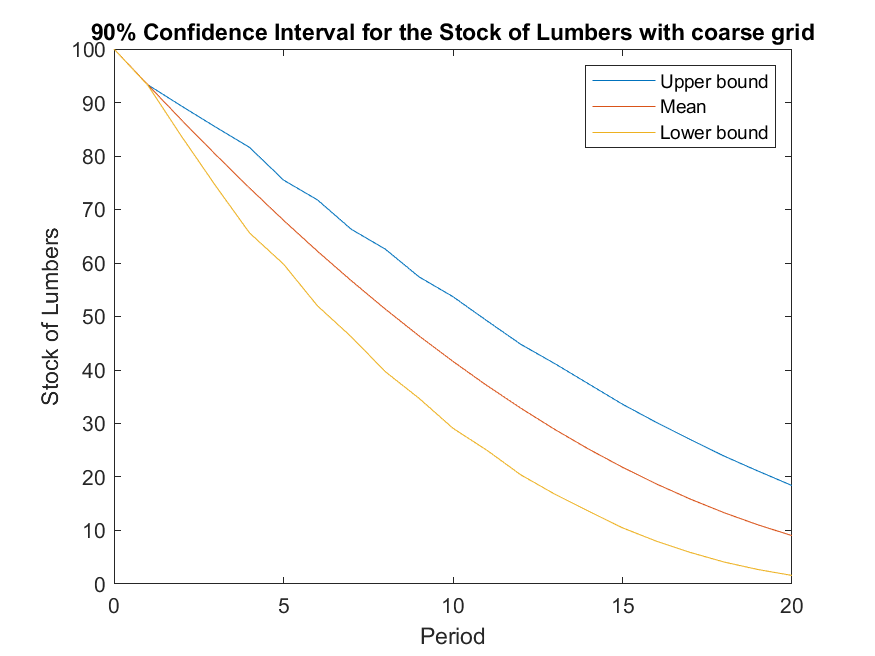
\includegraphics[width=\textwidth]{ci2.png}
\caption{Expected stock and 90\% confidence interval}
\end{figure}
\clearpage
\section*{Code}
\begin{verbatim}
% Motoaki Takahashi
% HW6 Econ 512

clear all
delta = 0.95;
p0 = 0.5;
rho = 0.5;
N = 1000;
k0 = 100; % initial stock of lumber
k = (k0/N):k0/N:k0;

sigmau = 0.1;

%% Question 2
Z = 21; % number of grid points
% Z = 5 % for coarse grid

 
 [prob,grid]=tauchen(Z,p0,rho,sigmau);
disp(['The dimensions of prob are ' num2str(size(prob)) ])
disp(['The dimensions of grid are ' num2str(size(grid)) ])

%% Question 3


v = zeros(N, Z); % initial guess for value function
decision = zeros(N,Z); % this will contain the firm's policy
newv = zeros(N,Z); % this will contain 

%% value function iteration

dif = 1;
tol = 1E-4;
while dif > tol
    EV = v * prob';
    for i = 1:N
        prof = kron(grid, k(i)*ones(N, 1)-k');
        prof(prof < 0) = -1E5; % punish a negative stock of lumber
        inv = k(i)*ones(N, 1)-k';
        inv(inv<0) = 0; % avoid generating an imaginary number
        inv = kron(ones(1, Z), inv);
        prof = prof - 0.2 * inv .^ (1.5); % subtract inv costs from the gross profits
        [vnew(i,:),decision(i,:)]=max(prof + delta * EV);

    end
   dif=norm(vnew-v)/norm(vnew);
   disp(dif)
   v=vnew;
end

%% 
plot(k, v(:, 8), k, v(:, 11), k, v(:, 14)) % for grid Z = 21
% plot(k, v(:, 2), k, v(:, 3), k, v(:, 4)) % for coarse grid Z = 5
title('Value function')
xlabel('Stock of lumber')
ylabel('Value')

%% Question 4

plot(grid, decision(1,:), grid, decision(101,:), grid, decision(201,:), grid, decision(301,:), grid, decision(401,:), grid, decision(501,:), grid, decision(601,:),grid, decision(701,:),grid, decision(801,:), grid, decision(901,:))

title('Next period stock vs lumber prices')
xlabel('Lumber price')
ylabel('Next period stock of lumber')

%% Question 5

% simulation
% let's run 1000 paths and numerically get the means and the confidence
% interval of stocks

p = 1; % the initial value of lumber
k0 = 100; % the initial stock of lumber

% we will get n = 1000 simulations
n = 1000;
numSteps = 21; % initial state is p=1 and 20 periods ahead

simu_price = zeros(n, numSteps); % this will contain the simulated paths of prices
simu_price(:, 1) = ((Z+1)/2) * ones(n, 1);

% make the cumulative version of the transition matrix
cumu = cumsum(prob, 2);

for s = 1:n
    for step = 2:21
        r = rand;
        simu_price(s, step) = find(cumu(simu_price(s, step-1),:) > r, 1);
    end
end

% Get the simulated paths of lumber stocks associated with the prices

simu_ind = zeros(n, numSteps);
simu_ind(:, 1) = N * ones(n, 1);
simu_cap = zeros(n, numSteps);
simu_cap(:, 1) = k0 * ones(n, 1);

for s = 1:n
    for step = 2:21
        simu_ind(s, step) = decision(simu_ind(s, step-1), simu_price(s, step-1));
        simu_cap(s, step) = k(simu_ind(s, step));
    end
end

meancap = mean(simu_cap);
secap = std(simu_cap) ./ sqrt(n);
ts = tinv([0.05  0.95], n-1); 

cicap = kron(meancap, ones(2, 1)) +  kron(ts', secap);
memori = 1:numSteps;
plot(memori, meancap, memori, cicap)

title('Mean and 90 percent CI for lumber stocks')
xlabel('Period')
ylabel('Stock of lumber')

%% Question 6

% for question 6, redo with Z = 5
\end{verbatim}
\end{document}